\section{Born formulation and induced-association sensitivity}

\subsection{Question and conditions}

The calculation crosses original Born versus shell-modified Born with
ion-suppressed relative permittivity against CO2--water induced association
off/on. Temperature, pressure, unloaded MEA mass fraction, and CO2 loadings are
\SI{313.15}{\kelvin}, \SI{101325}{\pascal}, 30 wt\%, and 0.11--0.99 mol
CO2/mol MEA. Neutral molecular parameters, five reaction correlations, and all
other ionic parameters remain fixed.

\subsection{Methods and sources}

Original-Born cases use solvent-only relative permittivity and
$c_{\mathrm{shell}}=c_{\mathrm{dielectric}}=0$. Shell-modified-Born cases use
$c_{\mathrm{shell}}=c_{\mathrm{dielectric}}=1$ together with the fixed
ion-fraction suppression coefficient 7.01. Six Jakobsen et al. (2005)
speciation states are evaluated. The Amundsen et al. (2009) unloaded density of
\SI{1003.4}{\kilogram\per\cubic\metre} is used only as a liquid-density scale.

\subsection{Fixed-parameter result}

\begin{table}[ht]
\centering
\caption{Born-formulation by induced-association sensitivity.}
\begin{tabular}{lrrr}
\toprule
Formulation & Evaluated & Density (kg/m$^3$) & Factor \\
\midrule
Original Born, association off & 2/6 & 1.087--1.125 & 2.531 \\
Original Born, association on & 2/6 & 1.087--1.125 & 2.531 \\
Shell Born, ion-suppressed, association off & 6/6 & 1065.5--1445.3 & 1.3235 \\
Shell Born, ion-suppressed, association on & 6/6 & 1065.5--1447.6 & 1.3238 \\
\bottomrule
\end{tabular}
\end{table}

\begin{figure}[ht]
\centering
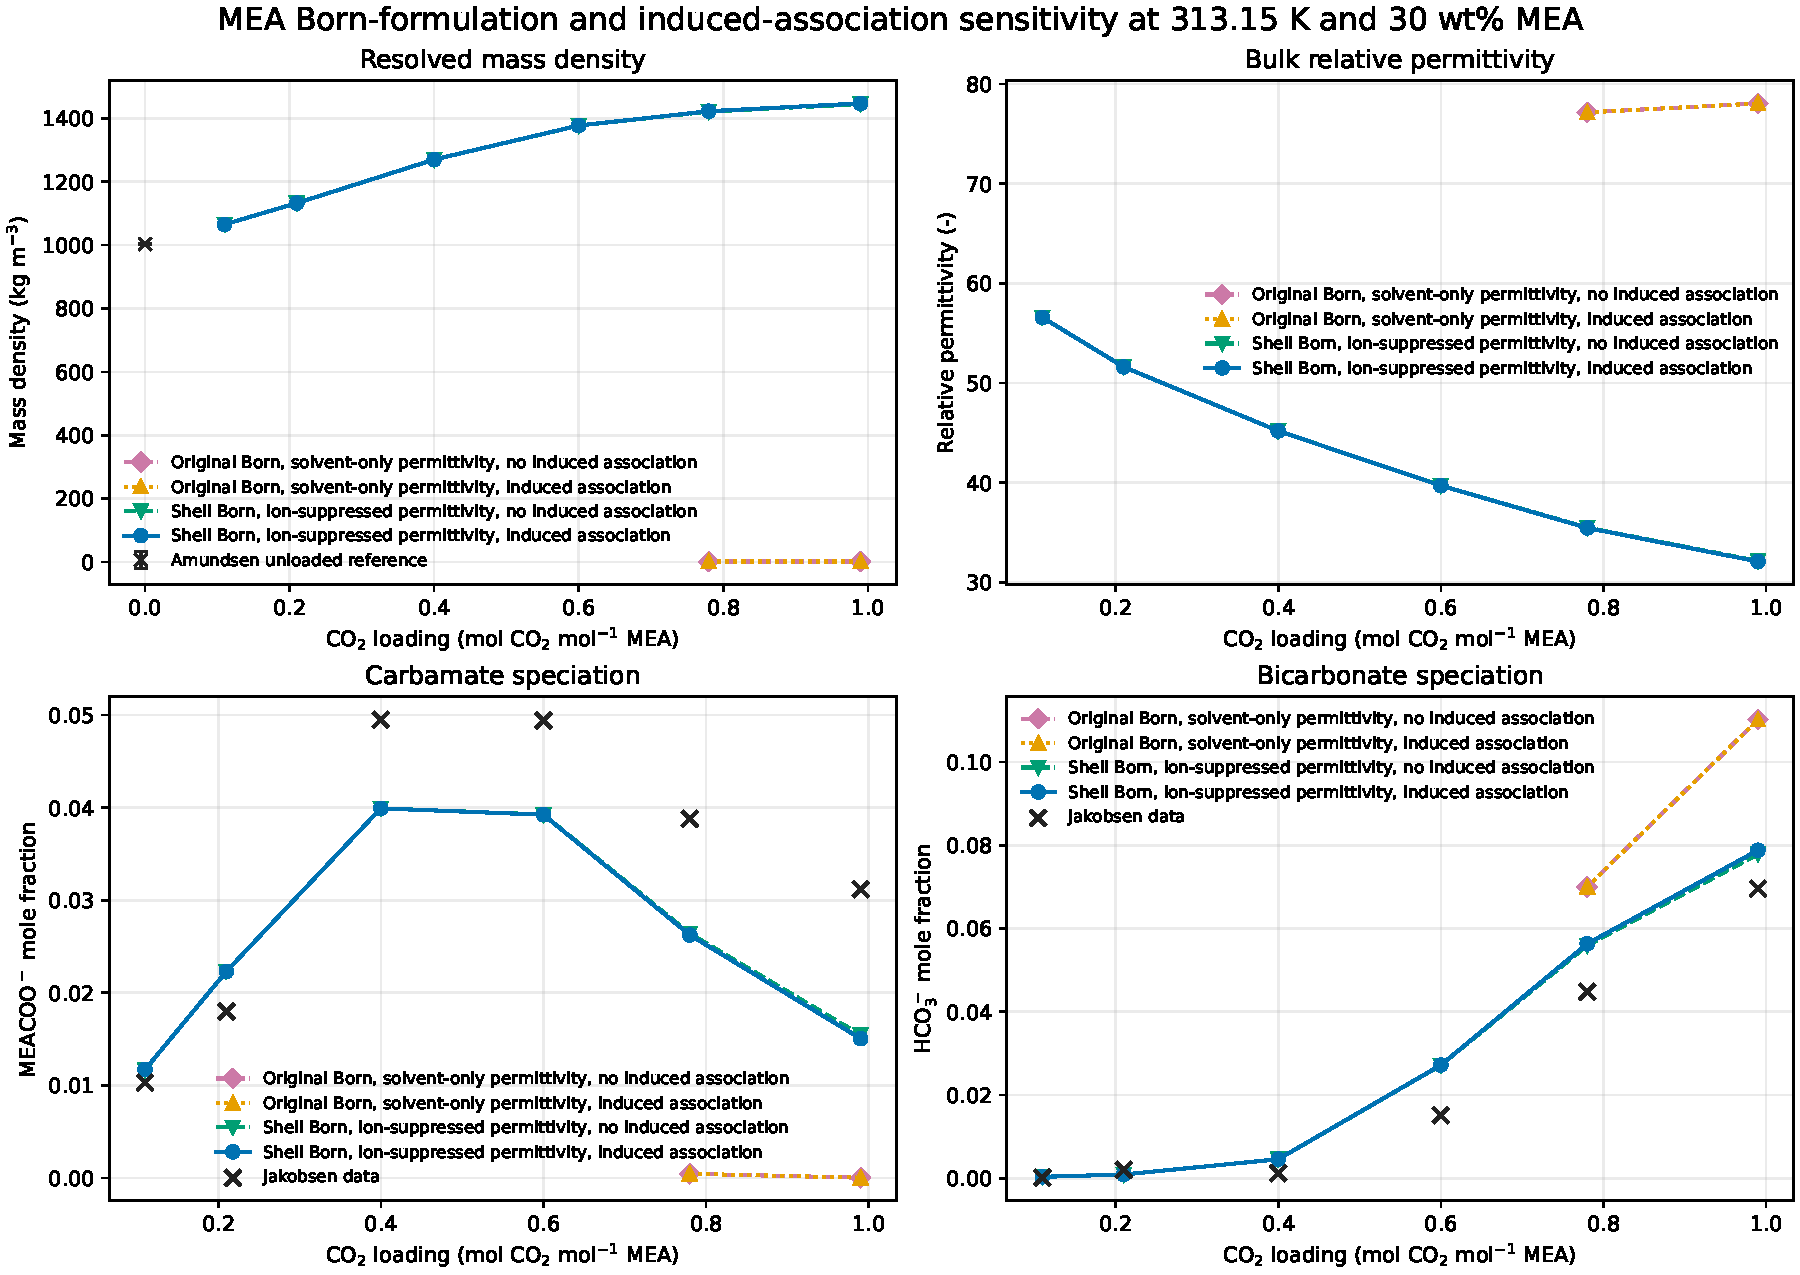
\includegraphics[width=0.98\textwidth]{analyses/phase3/ionic_epcsaft_regression/born_permittivity_sensitivity/figures/born_permittivity_sensitivity.pdf}
\caption{Resolved density, relative permittivity, and Jakobsen carbamate and
bicarbonate comparisons. Exact plotted values are retained with the analysis.}
\end{figure}

Both original-Born cases fail four states and return vapor-density roots for
the remaining two. Both shell-Born, ion-suppressed cases resolve all six
liquid-density states. Induced association changes their density by at most
\SI{2.27}{\kilogram\per\cubic\metre}; their fixed-parameter typical speciation
factors are 1.3235 and 1.3238.

\subsection{Two-ion-diameter result}

Only the protonated-MEA and carbamate-anion segment diameters are fitted. The
objective contains 32 unweighted natural-log residuals for direct-positive
Jakobsen observations. Aggregate rows are excluded. Original-Born cases are
not fitted because they supply no admissible liquid starting branch.

\begin{table}[ht]
\centering
\caption{Two-ion-diameter sensitivity fit under shell Born and ion-suppressed
relative permittivity.}
\begin{tabular}{lrrrr}
\toprule
Association & $\sigma_{\mathrm{MEAH^+}}$ (\AA) &
$\sigma_{\mathrm{MEACOO^-}}$ (\AA) & log SSE & Factor \\
\midrule
Off & 2.00000 & 3.07165 & 22.811 & 1.477 \\
On & 2.00000 & 3.06644 & 23.303 & 1.442 \\
\bottomrule
\end{tabular}
\end{table}

\begin{figure}[ht]
\centering
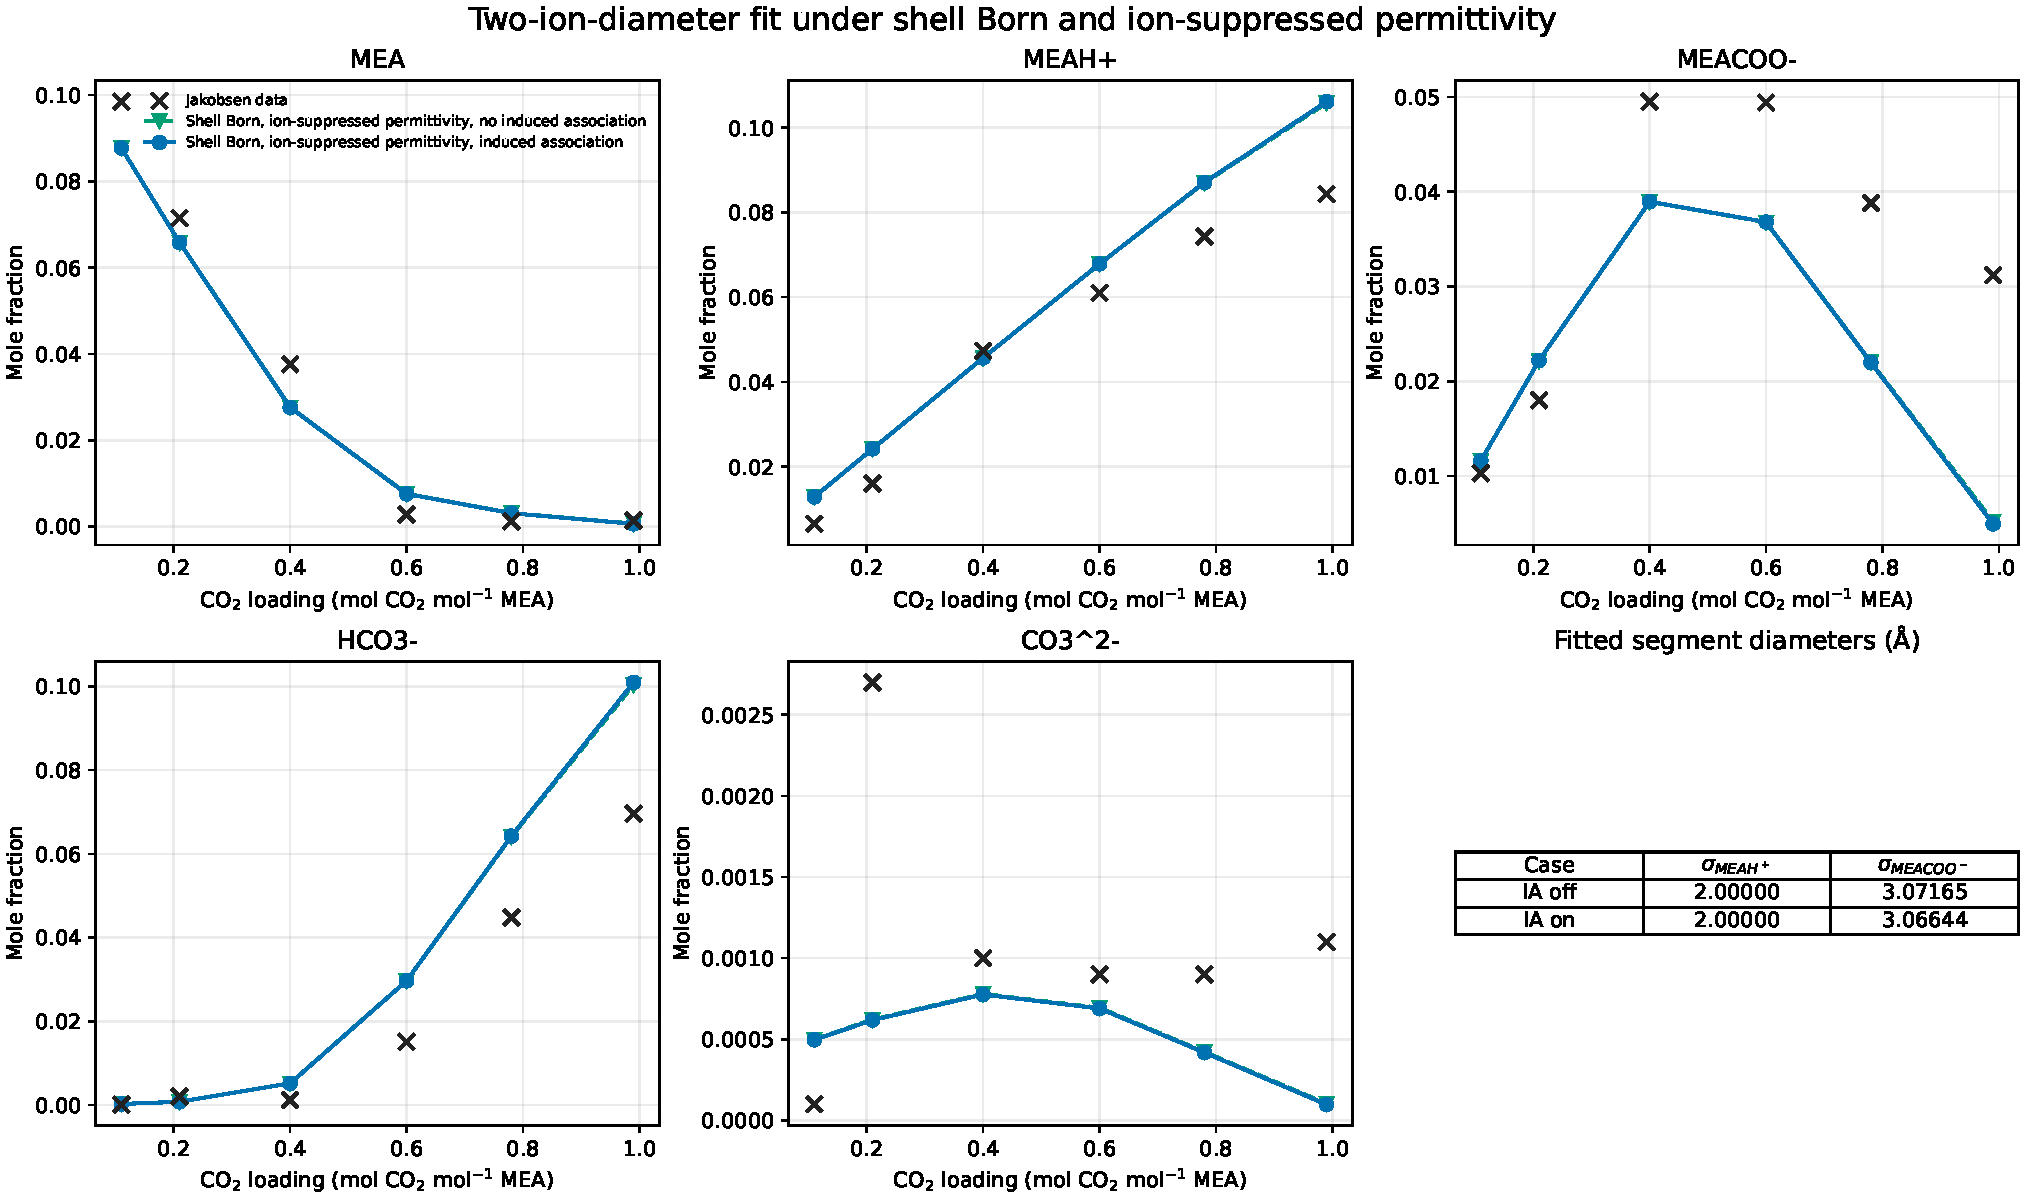
\includegraphics[width=0.98\textwidth]{analyses/phase3/ionic_epcsaft_regression/born_permittivity_sensitivity/figures/ion_diameter_fit.pdf}
\caption{Direct Jakobsen observations and fitted speciation values. The last
panel records the exact fitted segment diameters.}
\end{figure}

Both fits move the protonated-MEA diameter from \SI{3.48509}{\angstrom} to the
exploratory lower bound and the carbamate-anion diameter from
\SI{3.53544}{\angstrom} to approximately \SI{3.07}{\angstrom}. The two-column
Jacobian condition numbers are 3.23 and 3.21, so the boundary direction is not
caused by numerical rank deficiency. Induced association remains retained
because its separate CO2--water phase-equilibrium comparison supports it, even
though it is nearly neutral in this fixed-pressure speciation study.

These fits do not qualify a final parameter set: they cover one temperature
and solvent concentration, use no observation uncertainty weights, and place
the protonated-MEA diameter at the tested boundary. They identify the next
model/data discrepancy to resolve with broader pressure, speciation, density,
or independent ionic evidence.

\subsection{Independent ion-suppression coefficient blocks}

The coefficient study retains shell Born, ion-suppressed relative
permittivity, CO2--water induced association, $\alpha_{\mathrm{H_3O^+}}=9.55$,
and $\alpha_{\mathrm{OH^-}}=13.96$. Unsupported ions start at 7.01. The first
block changes $\alpha_{\mathrm{MEAH^+}}$ to 2.60 and
$\alpha_{\mathrm{MEACOO^-}}$ to 7.89 independently and together. The second
block applies the same independent comparison to bicarbonate and carbonate on
the best full-coverage amine base. No coefficient is fitted.

\begin{table}[ht]
\centering
\caption{Fixed ion-suppression coefficient sensitivity across all six
Jakobsen loading states.}
\begin{tabular}{lrr}
\toprule
Configuration & Evaluated & Typical factor \\
\midrule
Remaining ions 7.01 & 6/6 & 1.32380 \\
MEAH$^+$ = 2.60 & 6/6 & 1.28178 \\
MEACOO$^-$ = 7.89 & 6/6 & 1.32482 \\
MEAH$^+$ = 2.60; MEACOO$^-$ = 7.89 & 6/6 & 1.29242 \\
MEAH$^+$ = 2.60; HCO$_3^-$ = 7.89 & 6/6 & 1.27083 \\
MEAH$^+$ = 2.60; CO$_3^{2-}$ = 7.89 & 6/6 & 1.28067 \\
MEAH$^+$ = 2.60; HCO$_3^-$/CO$_3^{2-}$ = 7.89 & 6/6 & 1.26912 \\
\bottomrule
\end{tabular}
\end{table}

\begin{figure}[ht]
\centering
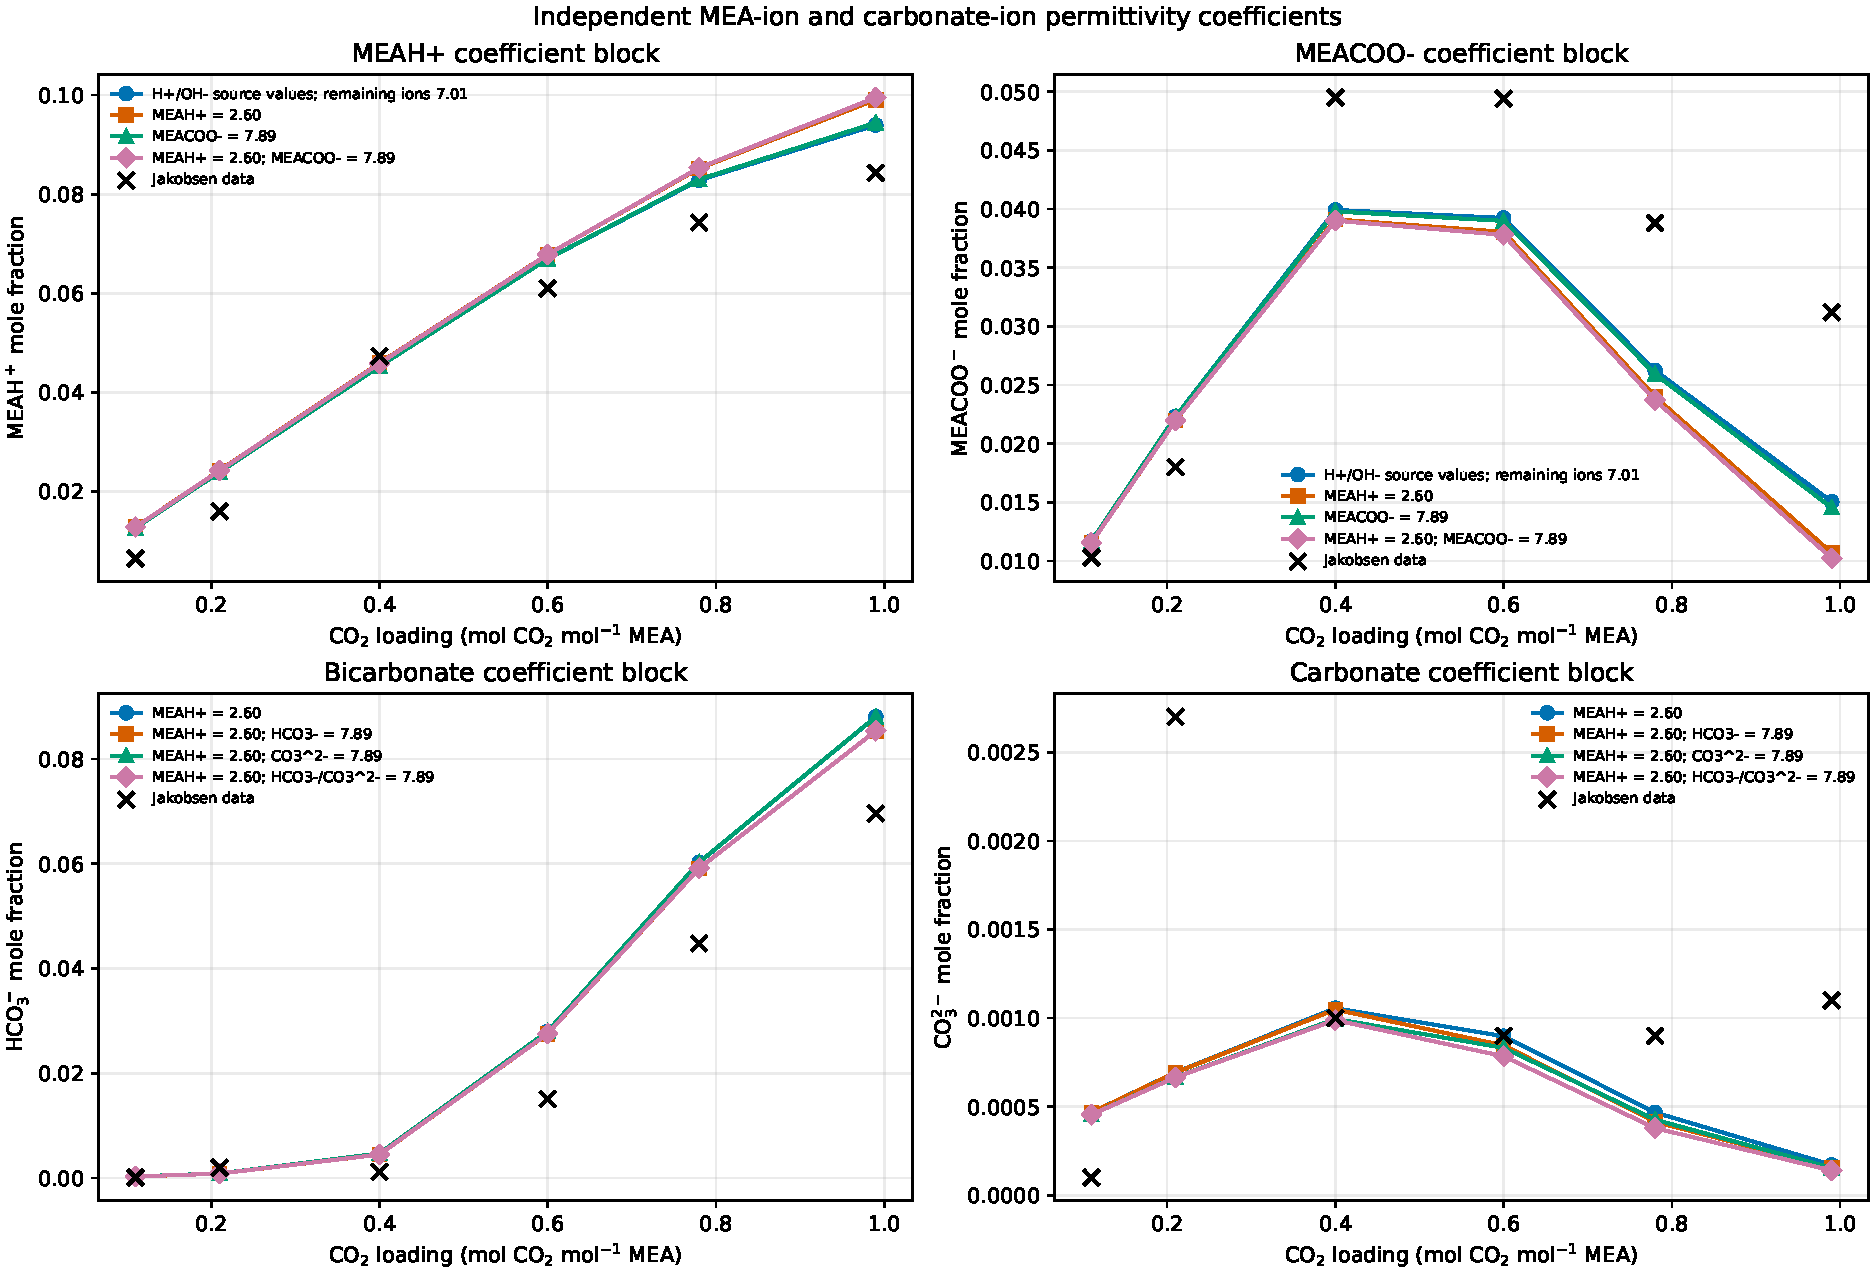
\includegraphics[width=0.98\textwidth]{analyses/phase3/ionic_epcsaft_regression/born_permittivity_sensitivity/figures/ion_coefficient_blocks.pdf}
\caption{Independent amine-ion and carbonate-ion coefficient changes against
the retained Jakobsen observations. Exact plotted values are retained in the
analysis results.}
\end{figure}

Changing the MEAH$^+$ coefficient is the controlling amine-ion perturbation;
MEACOO$^-$ alone is effectively neutral. Starting from MEAH$^+$ = 2.60,
bicarbonate supplies most of the additional median improvement and carbonate
alone is nearly neutral. Changing both carbonate coefficients gives the lowest
tested median factor, 1.26912, but increases the worst individual factor from
6.40 for the MEAH$^+$-only configuration to 7.85. The median improvement is
therefore not uniform across species. The MEAH$^+$ change primarily reduces
the molecular-CO2 and carbonate discrepancies while slightly worsening the
already closer MEAH$^+$ and MEACOO$^-$ predictions.

All 42 states evaluate. Maximum balance and reaction-affinity infinity norms
are $8.21\times10^{-16}$ and $2.84\times10^{-13}$. The calculation establishes
local sensitivity at \SI{313.15}{\kelvin} and 30 wt\% MEA; it does not identify
ion-specific coefficients from direct dielectric observations or establish
their transfer across temperature and solvent concentration.

\subsection{Broader temperature and pressure comparison}

The selected ion block was evaluated without regression against 15
source-backed 30 wt\% MEA pressure observations spanning 40--\SI{120}{\celsius}.
All structures retain shell Born, ion-suppressed permittivity, and CO2--water
induced association. The third structure replaces constant water permittivity
with the existing Archer--Wang temperature approximation.

\begin{table}[ht]
\centering
\caption{Broad fixed-structure comparison. Pressure errors use natural-log
model/observation residuals; Hajj errors are relative-permittivity units.}
\begin{tabular}{lrrrr}
\toprule
Configuration & Pressure & ln-RMSE & Factor & Hajj RMSE \\
\midrule
Remaining ions 7.01; constant $\epsilon_w$ & 7/15 & 6.802 & 4.398 & 32.80 \\
Selected ions; constant $\epsilon_w$ & 9/15 & 4.948 & 2.500 & 25.40 \\
Selected ions; $\epsilon_w(T)$ & 10/15 & 0.913 & 2.226 & 32.41 \\
\bottomrule
\end{tabular}
\end{table}

\begin{figure}[ht]
\centering
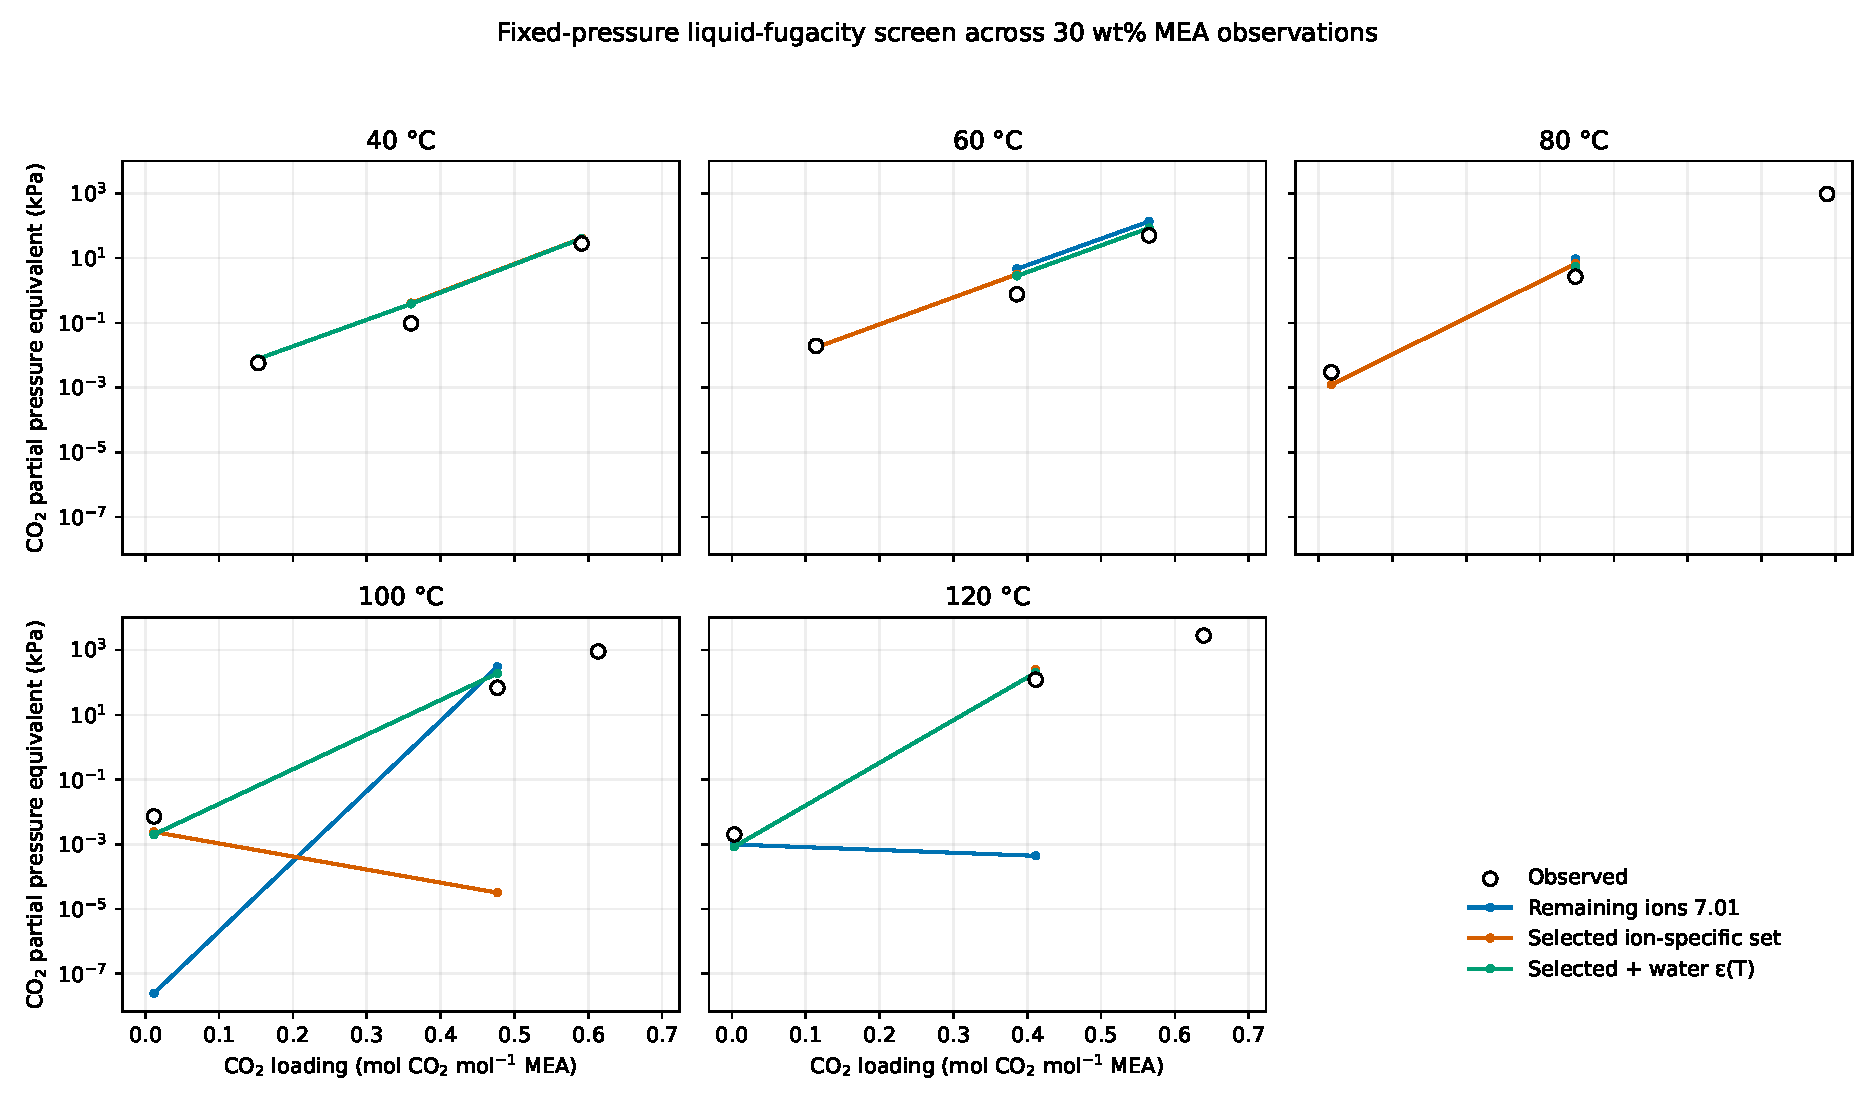
\includegraphics[width=0.98\textwidth]{analyses/phase3/ionic_epcsaft_regression/born_permittivity_sensitivity/figures/broader_candidate_pressure.pdf}
\caption{Diagnostic fixed-pressure neutral-CO2 liquid fugacity across the
five temperature profiles. Missing model markers are retained as explicit
non-evaluable states.}
\end{figure}

\begin{figure}[ht]
\centering
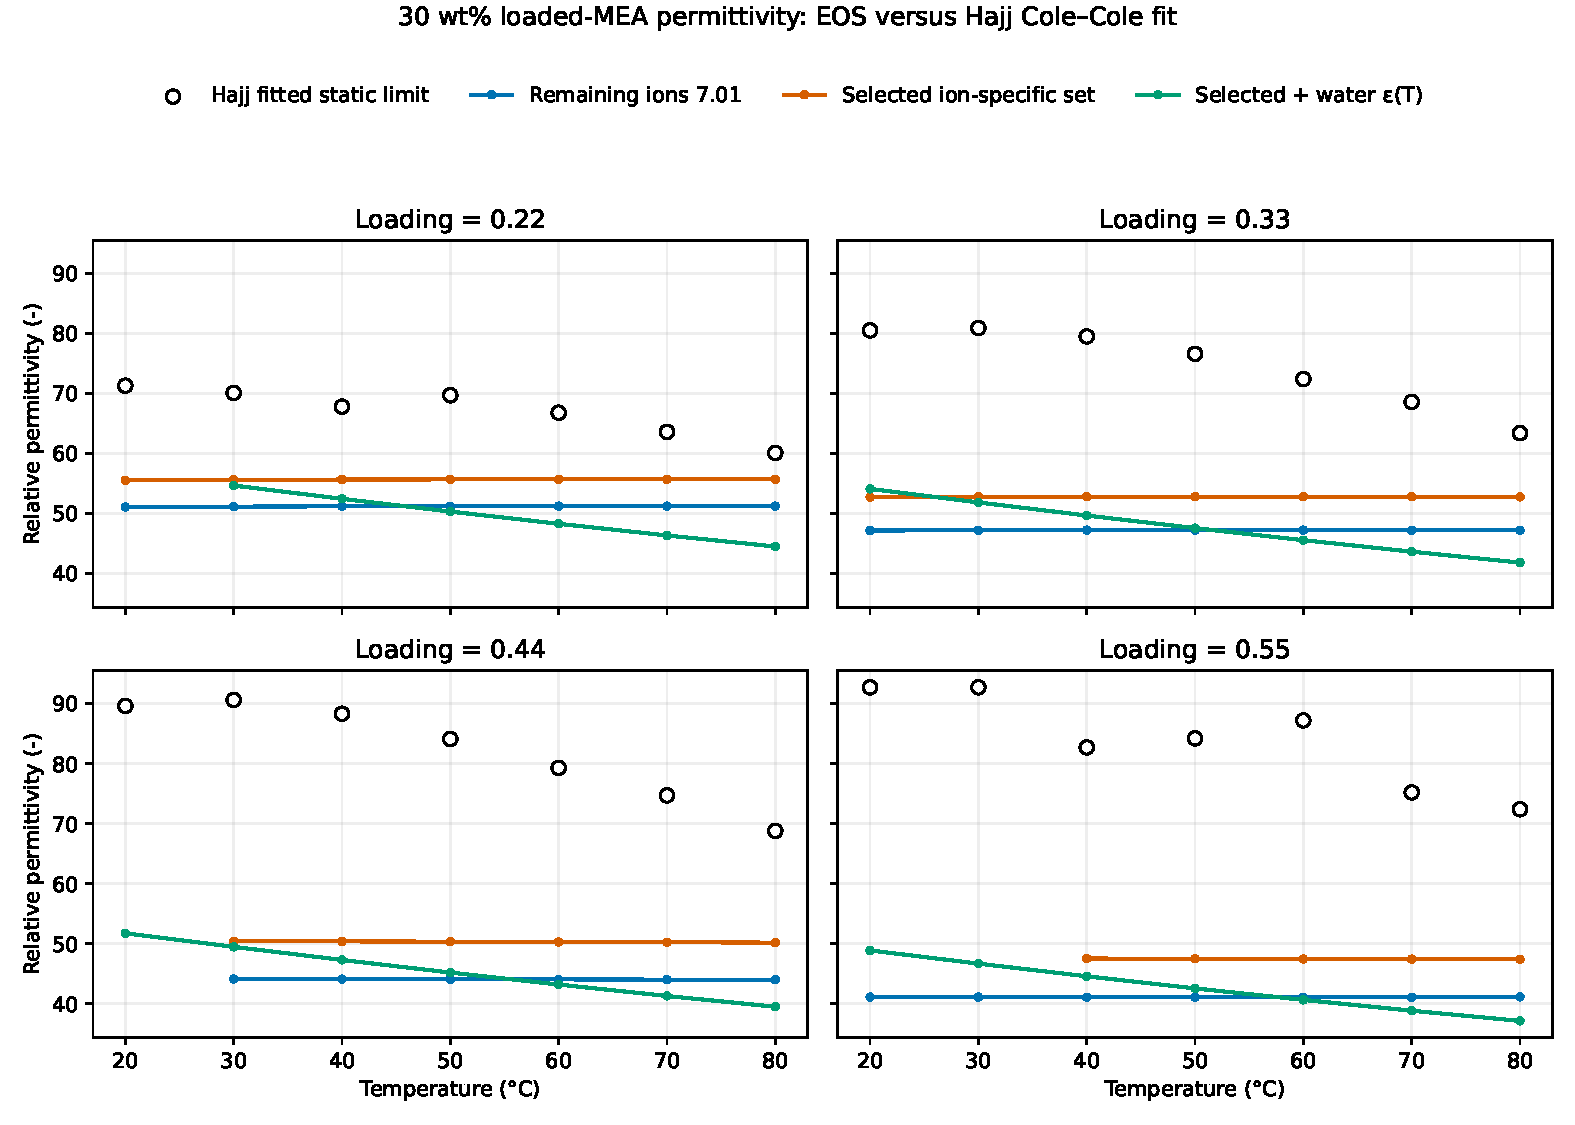
\includegraphics[width=0.98\textwidth]{analyses/phase3/ionic_epcsaft_regression/born_permittivity_sensitivity/figures/broader_candidate_dielectric.pdf}
\caption{EOS bulk relative permittivity against the Hajj et al. (2024)
Cole--Cole fitted static limit. The experimental quantity is an aggregate
microwave-fit limit, not a direct DC or single-ion permittivity.}
\end{figure}

The temperature-dependent water input removes the catastrophic pressure-error
branches among the evaluated states and gives the best broad pressure metric.
Its diagnostic pressure ln-RMSE is 0.913 and its typical factor is 2.226. A
representative \SI{40}{\celsius} coupled bubble calculation gives
\SI{406.37}{\pascal}, compared with \SI{407.49}{\pascal} from the diagnostic
liquid-fugacity calculation at the same state. The broad screen remains
limited by five non-evaluable states and by extrapolating the reaction
correlations above \SI{323.15}{\kelvin}.

The Hajj comparison does not independently identify the ion coefficients.
All structures underpredict its absolute fitted static limit, while
$\epsilon_w(T)$ provides the expected temperature direction. Direct
single-ion permittivity data do not exist for MEAH$^+$ and MEACOO$^-$ in this
model convention; analogous-ion support must instead come from mean ionic
activity, transfer, and solvation observables.

The best fixed starting document therefore combines
$\alpha_{\mathrm{MEAH^+}}=2.60$,
$\alpha_{\mathrm{MEACOO^-}}=7.01$,
$\alpha_{\mathrm{HCO_3^-}}=\alpha_{\mathrm{CO_3^{2-}}}=7.89$,
$\alpha_{\mathrm{H_3O^+}}=9.55$, and
$\alpha_{\mathrm{OH^-}}=13.96$ with the Archer--Wang water
$\epsilon(T)$ approximation. Its exact full mapping is retained in the broad
result directory as \texttt{best\_fixed\_candidate\_parameters.json}; the
complete mapping hash is recorded beside it in \texttt{summary.json}.
This selects the next regression starting structure; it is not yet a final
globally fitted parameter set.
